\chapter{Statistical learning theory}
\label{chap:slt}

\chapterprecishere{%
  To  understand  God's  thoughts  we  must study statistics, for these are the measure of His purpose.
  \par\raggedleft--- \textup{Florence Nightingale}, her diary}

We can address several kinds of problems using algorithms that learn from data.  However,
we focus on the problem of \emph{inductive learning}. Before we go further, let us define some terms.

\begin{defbox}{Artificial intelligence}{}
  The field that studies algorithms that exhibit intelligent behavior.
\end{defbox}

Artificial intelligence is a very broad field, including not only the study of algorithms
that exhibit intelligent behavior, but also the study of the behavior of intelligent
systems.  For instance, it encompasses the study of optimization methods, bioinspired algorithms,
robotics, philosophy of mind, and many other topics.  We are interested in the subfield of
artificial intelligence that studies algorithms that exhibit some form of intelligent
behavior.

\begin{defbox}{Machine learning}{}
  The subfield of artificial intelligence that studies algorithms that enable computers to
  automatically learn from data.
\end{defbox}

Machine learning is the subfield of artificial intelligence that studies algorithms that
enable computers to automatically learn and improve their performance on a task from
experience, without being explicitly programmed by a human being.

\begin{defbox}{Predictive learning}{}
  The machine learning paradigm that studies the problem of making predictions given known
  input data.
\end{defbox}

The machine learning paradigm that focuses on making predictions about outcomes (sometimes
about the future) based on historical data. Depending on the reasoning behind the learning
algorithms, the main predictive algorithms are classified in either inductive or
transductive.

\begin{defbox}{Inductive learning}{}
  The machine learning approach that involves deriving general rules from specific
  observations.
\end{defbox}

Induction a type of reasoning that goes from specific instances to more general
principles.  Inductive learning is the machine learning approach that studies algorithms
that, given data representing the set of specific instances, derive general rules that
can make predictions about \emph{any} new instances.

\Cref{fig:learning} give us a hierarchical view of the learning field.  Alternatives ---
such as descriptive learning in opposition to predictive learning, or transductive
learning in opposition to inductive learning --- are out of the scope of this course.

\begin{figurebox}[label=fig:learning]{Organizational chart of the learning field.}
  \centering
  \begin{tikzpicture}
    \draw[outline] (0,0) circle (30mm) node {};
    \node[below] at (0, 2.6) {artificial intelligence};
    \draw[outline] (0,-0.5) circle (25mm) node {};
    \node[below] at (0, 1.6) {machine learning};
    \draw[outline] (0,-1) circle (20mm) node {};
    \node[below] at (0, 0.5) {predictive learning};
    \draw[outline] (0,-1.5) circle (15mm) node {};
    \node[below] at (0, -1.0) {inductive learning};
  \end{tikzpicture}
  % \tcblower
  % Artificial intelligence is a very broad field, including not only the study of
  % algorithms that exhibit intelligent behavior, but also the study of the behavior of
  % intelligent systems.  Machine learning is a subfield of artificial intelligence that
  % studies algorithms that enable computers to automatically learn from data.  A particular
  % case of machine learning is predictive learning, which focuses on making predictions
  % about outcomes given known input data.  Inductive learning is a yet more specific type of
  % learning that involves deriving general rules from specific observations.
\end{figurebox}

Maybe the most general (and useful) framework for predictive learning is Statistical
Learning Theory.  In this chapter, we will introduce the basic concepts of this theory.

\section{Hypothesis and setup}

Consider the set
\begin{equation}
  \label{eq:training-set}
  \big\{(\vec{x}_i, y_i) : i = 1, \dots, n \big\}
\end{equation}
where each sample $i$ is associated with a feature vector $\vec{x}_i \in \mathcal{X}$ and a target variable
$y_i \in \mathcal{Y}$.  We assume that samples are random independent identically
distributed (i.i.d.) observations drawn according to $$\Prob(x, y) = \Prob(y \mid x) \Prob(x)\text{.}$$
Both $\Prob(x)$ and $\Prob(y \mid x)$ are fixed but unknown.

This is equivalent to the original learning problem stated by \textcite{Vapnik1999b}, where
a generator produce random vectors $\vec{x}$ according to a fixed but unknown
probability distribution $\Prob(x)$ and a supervisor returns an output value $y$ for every
input vector $x$ according to a conditional distribution function $\Prob(y \mid x)$, also fixed but
unknown.

Moreover, note that this setup is compatible with the idea of tidy data and 3NF (see
\cref{sub:bridge}). Of course, we assume $X, Y$ are only the measured variables (or
non-prime attributes).  In practice, it means that we left aside the keys in the learning
process.

\section{The learning problem}

Consider a \emph{learning machine} capable of generating a set of functions $f(x;
\theta) \equiv f_\theta(x)$, $\theta \in \Theta$ and $f_\theta : \mathcal{X} \rightarrow \mathcal{Y}$.
The problem of learning is that of choosing, among all possible $f_\theta$, the one that
predicts the target variable the best possible way.

In order to learn, we must first define the \emph{loss} (or discrepancy) $\mathcal{L}$
between the response $y$ to a given input $x$, drawn from $\Prob(x, y)$, and the
response provided by the learning machine.

Then, given the \emph{risk function}
\begin{equation}
  \label{eq:risk}
  R(\theta) = \int \mathcal{L}(y, f_\theta(x))\, d\Prob(x, y)\text{,}
\end{equation}
the goal is to find the function $f_\theta$ that minimizes $R(\theta)$
where the only available information is the \emph{training set} \eqref{eq:training-set}.
This is the \emph{empirical risk minimization} (ERM) problem.

This formulation encompasses many specific problems. I focus on the two of them which I
believe are the most fundamental ones: \emph{binary data classification}\footnote{Vapnik
calls it \emph{pattern recognition}.} and \emph{regression estimation}\footnote{We are not
talking about \emph{regression analysis}, it is closer to the \emph{scoring} task
definition by \textcite{Zumel2019}.}.  I left aside the density estimation problem, once
it is not
addressed in the remaining of the book.

\paragraph{Binary data classification task.}  In this task, the output $y$ take on
only two possible values, zero or one --- called classes ---, and the functions $f_\theta$ are indicator
functions. For the loss
\begin{equation*}
  \mathcal{L}(y, f_\theta(x)) = \begin{cases}
    0 & \text{if } y = f_\theta(x) \\
    1 & \text{if } y \neq f_\theta(x)\text{,}
  \end{cases}
\end{equation*}
we aim at minimizing the risk $\eqref{eq:risk}$ which becomes the probability of
classification error.  The function $f$, in this case, is called \emph{classifier}.

\paragraph{Regression estimation task.} Let the outcome $y$ be a real value and
the \emph{regression} $r$ be $$r(x) = \int y\, d\Prob(y|x) \text{.}$$

The regression function is the function $r = f_\theta$ that minimizes the risk function
\eqref{eq:risk} with the loss
\begin{equation*}
  \mathcal{L}(y, f_\theta(x)) = \big(y - f_\theta(x)\big)^2\text{.}
\end{equation*}

If $r \not\in \left\{ f_\theta : \theta\in\Theta \right\}$, the function $f_{\theta'}$
that minimizes the risk function is the closest to the regression function in the
metric $l_2$, i.e. we look for $\theta'$ such that
\begin{equation*}
  \theta' = \argmin_{\theta \in \Theta} \sqrt{
    \int \big(r(x) - f_\theta(x)\big)^2\, d\Prob(x)
  }\text{.}
\end{equation*}
The function $f$, in this case, is called \emph{regressor}.

\subsection{A few remarks and definitions}

\paragraph{Supervised and semisupervised learning}
In both cases, classification and regression, the learning task is to find the function
that maps the input data to the output data in the best possible way.  Although the
learning machine described generate models in a \emph{supervised} manner, there are
alternative ways to solve the inductive learning problem, such as \emph{semisupervised}
approach, where the model can be trained with a small subset of labeled data and a large
subset of unlabeled data --- that is, data whose labels $y$ are unknown.

\paragraph{Mislabeled data}
Another important premise is that all given labels are correct.  This is a strong
assumption, but it is necessary to ensure the learning process.  In practice, it is
possible to have mislabeled data, but it is a different problem that must be addressed
before the learning process.  Some works address the robustness of learning machines
in cases of mislabeled data \parencite{Silva2013}. % TODO more papers

\paragraph{Generative and discriminative models}
Any learning machine generates a model that describes the relationship between the input
and output data.  This model can be generative or discriminative.  Generative models
describe the joint probability distribution $\Prob(x, y)$ and can be used to generate new
data.  Discriminative models, on the other hand, describe the conditional probability
distribution $\Prob(y \mid x)$ and are used to make predictions. Generative models are
usually much more complex than discriminative models, but they hold more information about
the data, solving indirectly the conditional probability.  As a general rule, if you only
need to solve the predictive problem, use a discriminative model.

\paragraph{Multiclass classification}
In the binary classification task, the output $y$ is
a binary variable.  However, it is possible to have a multiclass classification task,
where  $y$ can take on more than two possible values.  Although some learning methods can
address directly the multiclass classification task, it is possible to transform the
problem into a binary classification task.  The most common method is the
\emph{one-versus-all} method where we train $l$ binary classifiers, one for each class,
and the class with the highest score is the predicted class.  Another method is the
\emph{one-versus-one} method, where we train $l(l-1)/2$ binary classifiers, one for each
pair of classes, and the class with the most votes is the predicted class.

\paragraph{Number of inputs and outputs}
Note that the definition of the learning problem does not restrict the number of inputs
and outputs.  The input data can be a scalar, a vector, a matrix, or a tensor, and the
output as well.  The learning machine must be able to handle the input and output data
according to the problem.

\paragraph{Parametric vs nonparametric models}
The learning machine generates a set of functions $f_\theta$ where $|\theta|$ can be fixed
or not.  If $|\theta|$ is always fixed, the model is called \emph{parametric}.  If
$|\theta|$ is not fixed beforehand, the model is called \emph{nonparametric}.  Parametric
models are usually simpler and faster, but they are less flexible.  In other words, it is
up to the researcher to choose the best model ``size'' for the problem.  If the model is
too small, it will not be able to capture the complexity of the data.  If the model is too
large, it will be too complex, too slow to train and might overfit to the data. Non
parametric models are more flexible, but they usually require more data to be trained.

\section{ERM inductive principle}

In the following sections, $z$ describes the pair $(x, y)$ and $L(z, \theta)$ a generic loss
function.  The training dataset is thus a set of $n$ i.i.d. samples $z_1, \dots, z_n$.

Since the distribution $\Prob(z)$ is unknown, the risk functional $R(\theta)$ is replaced by
the \emph{empirical risk functional}
\begin{equation}
  \label{eq:empirical-risk}
  R_n(\theta) = \frac{1}{n} \sum_{i=1}^n L(z_i, \theta)\text{.}
\end{equation}

Approximating $R(\theta)$ by the empirical risk functional $R_n(\theta)$ is the so called
ERM inductive principle.  The ERM principle is the basis of the statistical learning
theory.

Classical methods, such as least-squares, maximum likelihood, and maximum a posteriori are
all realizations of the ERM principle for specific loss functions and hypothesis spaces.

In the following sections, we address the four main questions of learning theory.  We
summarize them in \cref{tab:learning-questions}.

\begin{tablebox}[label=tab:learning-questions]{The four main questions of learning theory.}
  \begin{tabularx}{\textwidth}{@{}lX@{}}
    \toprule
    Part & Question \\
    \midrule
    \textbf{Consistency} &
      What are the necessary and sufficient conditions for consistency of a learning process? \\
    \textbf{Rate of convergence} &
      How fast is the rate of convergence of the learning process? \\
    \textbf{Generalization} &
      How can one controle the generalization ability of the learning process? \\
    \textbf{Construction} &
      How can one construct a learning machine that satisfies the conditions of consistency and generalization? \\
    \bottomrule
  \end{tabularx}
\end{tablebox}

\section{Consistency of learning processes}

Addressing consistency of a learning process means that we are interested in the
convergence of the empirical risk functional $R_n(\theta)$ to the risk functional
$R(\theta)$ as $n \to \infty$.  In other words, it is an asymptotic theory about the
behavior of the empirical risk functional as the sample size $n$ goes to infinity.

The necessary and sufficient conditions for consistency give us guarantees that the learning
process is general and cannot be improved given our premises.  The most important topic in
this section is the Vapnik-Chervonenkis (VC) entropy.

\subsection{Definition of consistency}

An ERM method is consistent if it produces a sequence of functions $f_{\theta_n}$, for
$n = 1, 2, \dots$, for which both the expected risk and the empirical risk converge to the
their minimum values.

\begin{defbox}{Consistency of a learning process}{}
  Let $\theta_n$ be the solution of
  \begin{equation*}
    \theta_n = \argmin_{\theta \in \Theta} R_n(\theta)\text{.}
  \end{equation*}

  An ERM method is consistent for the set of functions $\left\{ L(z, \theta) : \theta \in
  \Theta \right\}$ and the probability distribution $\Prob(z)$ if
  \begin{align*}
    \lim_{n \to \infty} R(\theta_n) &= \inf_{\theta \in \Theta} R(\theta)\text{,} \\
    \lim_{n \to \infty} R_n(\theta_n) &= \inf_{\theta \in \Theta} R(\theta)\text{.}
  \end{align*}
\end{defbox}

This definition means that one can estimate the risk functional $R(\theta)$ by the
empirical risk functional $R_n(\theta)$, while the values of achieved risks converge to
the minimum value of the risk functional.  See \cref{fig:consistency}.

\begin{figurebox}[label=fig:consistency]{Convergence of the empirical and expected risk functionals.}
  \centering
  \begin{tikzpicture}
    \begin{axis}[
        ticks=none,
        axis x line=bottom,
        axis y line=left,
        ymin=0,
        ymax=11,
        xlabel={$n$},
        legend pos=south east,
        legend style={draw=none, fill=none},
        width=0.9\textwidth,
        height=0.6\textwidth,
      ]
      \addplot+[smooth, mark=none, black] coordinates {
        (1, 10) (2, 6) (3, 5) (5, 4.1)
      };
      \addlegendentry{$R(\theta_n)$}
      \addplot+[smooth, mark=none, dashed, black] coordinates {
        (1, 0) (2, 0.1) (3, 3) (5, 3.9)
      };
      \addlegendentry{$R_n(\theta_n)$}
      \draw[dotted, gray] (axis cs:6, 4) -- (axis cs:-1, 4);
    \end{axis}
    \node[gray] at (1, 1.8) {$\inf_{\theta \in \Theta} R(\theta)$};
  \end{tikzpicture}
\end{figurebox}

However, since this definition of consistency includes cases of trivial consistency, there
is no way to obtain such conditions.

Consider the following example.  Suppose we have found a set of functions $\left\{ f_\theta
: \theta \in \Theta \right\}$ such that the ERM method is not consistent.  Let's add
one more function $\phi(z)$ to the set, such that
\begin{equation*}
  \inf_{\theta \in \Theta} L(z, \theta) > \phi(z),~\forall z\text{.}
\end{equation*}
It is straightforward to see that the ERM method is consistent for the new set of
functions $\left\{ L(z, \theta) : \theta \in \Theta \right\} \cup \left\{ \phi \right\}$
and the probability distribution $\Prob(z)$.  In this case, the function $\phi(z)$ gives both
the minimum value of the risk functional and the empirical risk functional.  This is
illustrated in \cref{fig:trivial-consistency}.

% A tikz picture showing the senoidal functions L(z, theta) and phi(z) and the infimum of
% the risk functionals.
\begin{figurebox}[label=fig:trivial-consistency]{An illustrative case of trivial consistency.}
  \centering
  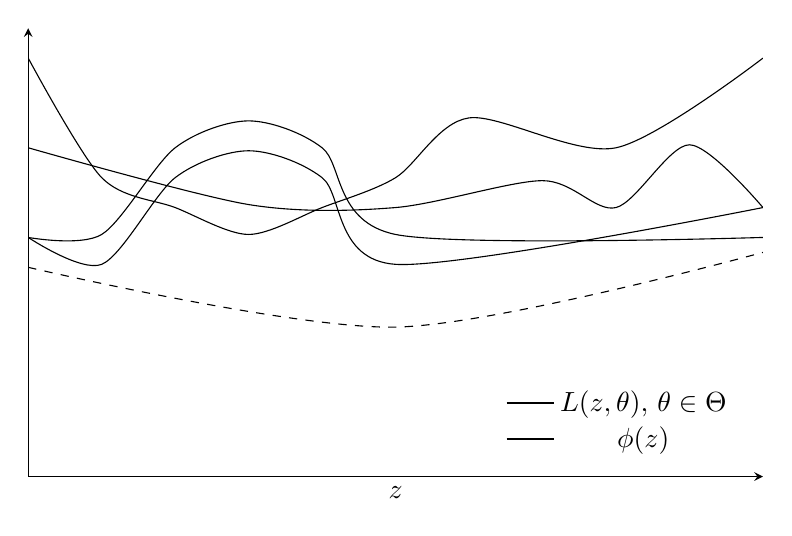
\begin{tikzpicture}
    \begin{axis}[
        ticks=none,
        axis x line=bottom,
        axis y line=left,
        ymin=-4,
        ymax=11,
        xlabel={$z$},
        legend pos=south east,
        legend style={draw=none, fill=none},
        width=0.9\textwidth,
        height=0.6\textwidth,
      ]
      \addplot+[smooth, mark=none, black] coordinates {
        (0, 10) (1, 6) (2, 5) (3, 4.1) (4, 5) (5, 6) (6, 8) (8, 7) (10, 10)
      };
      \addplot+[smooth, mark=none, black] coordinates {
        (0, 4) (1, 4.1) (2, 7) (3, 7.9) (4, 7) (5, 4.1) (10, 4)
      };
      \addplot+[smooth, mark=none, black] coordinates {
        (0, 4) (1, 3.1) (2, 6) (3, 6.9) (4, 6) (5, 3.1) (10, 5)
      };
      \addplot+[smooth, mark=none, black] coordinates {
        (0, 7) (3, 5.1) (5, 5) (7, 5.9) (8, 5) (9, 7.1) (10, 5)
      };
      \addlegendentry{$L(z, \theta)$, $\theta \in \Theta$}
      \addplot+[smooth, mark=none, black, dashed] coordinates {
        (0, 3) (5, 1) (10, 3.5)
      };
      \addlegendentry{$\phi(z)$}
    \end{axis}
  \end{tikzpicture}
\end{figurebox}

\subsection{Nontrivial consistency}


\section{Rate of convergence of learning processes}

\section{Generalization ability of learning processes}

\section{Construction of learning machines}

\subsection{Data classification methods}

\subsection{Regression estimation methods}
